\documentclass[12pt]{article}%
\usepackage{amsfonts}
\usepackage{fancyhdr}
\usepackage{comment}
\usepackage[a4paper, top=2.5cm, bottom=2.5cm, left=2.2cm, right=2.2cm]%
{geometry}
\usepackage{times}
\usepackage{amsmath}
\usepackage{changepage}
\usepackage{amssymb}
\usepackage{graphicx}%
\setcounter{MaxMatrixCols}{30}
\newtheorem{theorem}{Theorem}
\newtheorem{acknowledgement}[theorem]{Acknowledgement}
\newtheorem{algorithm}[theorem]{Algorithm}
\newtheorem{axiom}{Axiom}
\newtheorem{case}[theorem]{Case}
\newtheorem{claim}[theorem]{Claim}
\newtheorem{conclusion}[theorem]{Conclusion}
\newtheorem{condition}[theorem]{Condition}
\newtheorem{conjecture}[theorem]{Conjecture}
\newtheorem{corollary}[theorem]{Corollary}
\newtheorem{criterion}[theorem]{Criterion}
\newtheorem{definition}[theorem]{Definition}
\newtheorem{example}[theorem]{Example}
\newtheorem{exercise}[theorem]{Exercise}
\newtheorem{lemma}[theorem]{Lemma}
\newtheorem{notation}[theorem]{Notation}
\newtheorem{problem}[theorem]{Problem}
\newtheorem{proposition}[theorem]{Proposition}
\newtheorem{remark}[theorem]{Remark}
\newtheorem{solution}[theorem]{Solution}
\newtheorem{summary}[theorem]{Summary}
\newenvironment{proof}[1][Proof]{\textbf{#1.} }{\ \rule{0.5em}{0.5em}}

\newcommand{\Q}{\mathbb{Q}}
\newcommand{\R}{\mathbb{R}}
\newcommand{\C}{\mathbb{C}}
\newcommand{\Z}{\mathbb{Z}}

\begin{document}

\title{CS280 Spring 2025 Assignment 3 \\ Part A}
\author{RNN and LSTM}
\maketitle

\paragraph{Name: Chen Xuanxin}

\paragraph{Student ID: 2024233125}

\newpage


\subsubsection*{1. RNN (10 points)}
Assume that there is a simple RNN with all the variables as scalars. The hidden state $s_t$ at time step $t$ is computed from the previous hidden state $s_t$ and the current input $x_t$ as follows: 
$$s_t = \text{step}(w_1x_t+w_2s_{t-1}+b),$$
where $ \text{step}(z)=\left\{
	\begin{array}{ll}
	  1,\ z>0\\
	  0,\ \text{otherwise}\\
	\end{array}
  \right. $. The output is $y_t=s_t$.
\\\\\\
\noindent (a) Assuming $s_0 = 0$, please provide the values of $w_1$, $w_2$ and $b$ that could generate the output sequence
$$[0, 0, 0, 1, 1, 1, 1]$$
given the input sequence
$$[0, 0, 0, 1, 0, 1, 0].$$
\\

\noindent (b) Suppose that we want a model to generate the output sequence
$$[1, 1, 1, 0, 0, 0, 1, 1]$$
given the input sequence
$$[0, 0, 0, 1, 0, 0, 1, 0].$$
Do you think it is possible to use the above RNN to implement the mapping from the input sequence to the output sequence? If you answered ``no", please explain why. If you answered ``yes", please provide the parameters $w_1$, $w_2$, and $b$ required to implement the mapping.
		
\newpage

\subsubsection*{Answer 1}

\textbf{1.} The output shape is given by the formula:

\[
\text{Output size} = \frac{\text{Input size} - \text{Filter size} + 2 \times \text{Padding}}{\text{Stride}} + 1
\]

Thus, we have:

\[
\frac{64 - 6 + 2\times 1}{2} + 1 = \frac{60}{2} + 1 = 31
\]

The output shape is $31 \times 31 \times 10$.

Number of parameters (weights + biases):

Each filter: $6 \times 6 \times 10 = 360$ parameters.  

Total weights for 10 filters: $360 \times 10 = 3600$ parameters.  

Biases for each filter: $10$ parameters.

Therefore, total parameters: $3600 + 10 = 3610$.

\vspace{1em}

\textbf{2.} Yes, it is possible. Two successive convolutional layers, each with filter size $5\times 5$, stride 1 and padding 0, can be represented as a single convolutional layer. The equivalent single convolution filter size will be:

\[
(5 + 5 - 1) \times (5 + 5 - 1) = 9 \times 9
\]

Thus, the equivalent single filter size is $9 \times 9$.

\vspace{1em}

\textbf{3.} Yes, pooling layers do cause loss of information because they aggregate local spatial information. However, pooling layers are still widely used because:

(1) Pooling reduces the spatial dimension of feature maps, significantly decreasing computational cost and memory usage.

(2) Pooling layers provide a form of spatial invariance, making the CNN less sensitive to small translations or variations in input.



\newpage

\subsubsection*{2. LSTM (10 points)}
	\setlength{\itemsep}{-1pt}
	\setlength{\parsep}{0pt}
	\setlength{\parskip}{0pt}
Consider a standard LSTM unit as shown below. Assume that \( L \) is the loss function.  Given the gradient \( \frac{\partial L}{\partial c_t}\) (backpropagated directly from \( c_{t+1} \)  to \( c_{t}\)) and the gradient \( \frac{\partial L}{\partial h_t}\), compute the following gradients: \( \frac{\partial L}{\partial x_t} \) and \( \frac{\partial L}{\partial h_{t-1}} \). Please provide a complete mathematical derivation and clearly present the formulas for each step.
	\begin{figure}[h]
		\centering
		\begin{minipage}{0.4\textwidth}
			\centering
			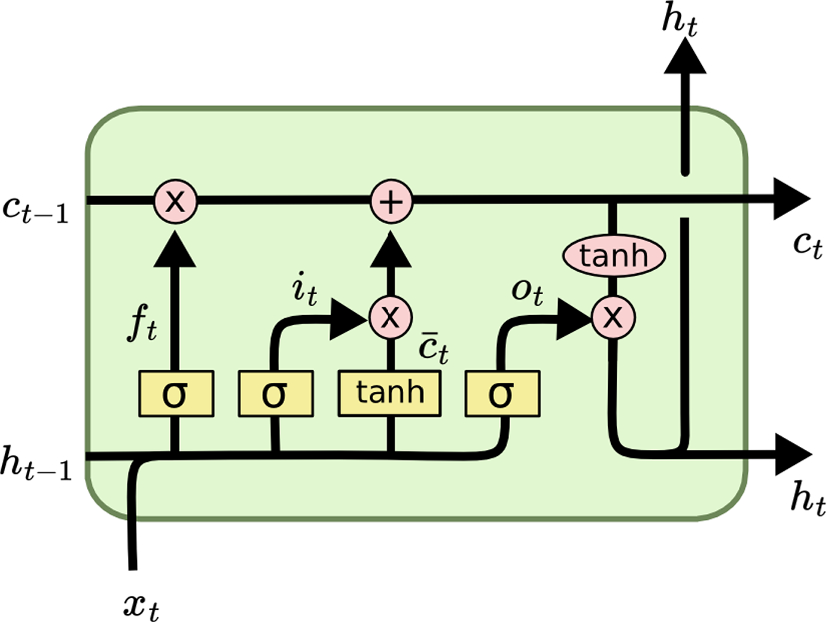
\includegraphics[width=\textwidth]{lstm.png} 
			\caption{LSTM unit}
			\label{fig:lstm}
		\end{minipage}
		\hfill
		\begin{minipage}{0.5\textwidth}
			\centering
			\begin{align*}
				i_t &= \sigma(W_i x_t + U_i h_{t-1} + b_i) \\
				f_t &= \sigma(W_f x_t + U_f h_{t-1} + b_f) \\
				o_t &= \sigma(W_o x_t + U_o h_{t-1} + b_o) \\
				\bar{c_t} &= \tanh(W_c x_t + U_c h_{t-1} + b_c) \\
				c_t &= f_t \odot c_{t-1} + i_t \odot \bar{c_t} \\
				h_t &= o_t \odot \tanh(c_t)
			\end{align*}
		\end{minipage}
	\end{figure}\\

\newpage

\subsubsection*{Answer 2}

\textbf{1.} My answer is as follows:

Function $F(z, w)$ is the forward convolution function that convolves input image $z$ with kernel $w$ to produce the output feature map $x$. It is necessary because it computes the output activations for forward propagation.

Function $G(\epsilon)$ is the backward convolution (gradient) function. It computes gradients of the loss with respect to inputs $z$ (denoted as $g_z$) and weights $w$ (denoted as $g_w$), given the upstream gradient $\epsilon$. It is needed to perform the backward propagation (training) to update parameters using gradients.

\vspace{1em}

\textbf{2.} Shapes are as follows:

 (1) $x$: $(126, 126)$, since $128 - 3 + 1 = 126$.
 
 (2) $\epsilon$: Same as $x$, thus $(126, 126)$.
 
 (3) $g_z$: Same shape as original input $z$, thus $(128, 128)$.
 
 (4) $g_w$: Same shape as convolution kernel $w$, thus $(3, 3)$.
  
\vspace{1em}

\textbf{3.} My answer is as follows:
\begin{itemize}
 \item \textbf{Forward pass computational cost:}

Output dimension: $126\times126$, each position involves a $3\times3$ convolution operation, thus:

Multiplications per output pixel: $3 \times 3 = 9$  
Additions per output pixel: $9 - 1 = 8$

Total multiplications: $126 \times 126 \times 9 = 142,884$  
Total additions: $126 \times 126 \times 8 = 126,112$

 \item \textbf{Backward pass computational cost for $g_w$:}

Gradient $g_w$ has size $3\times3$. Each parameter of $g_w$ is computed by convolution of input $z$ (size $128\times128$) and gradient $\epsilon$ (size $126\times126$):

Total multiplications: same as forward pass, $126\times126\times9=142,884$  
Total additions: $126\times126\times8=126,112$

\end{itemize}

\end{document}